\documentclass[12pt,letterpaper,noanswers]{exam}
\usepackage[usenames,dvipsnames,svgnames,table]{xcolor}
\usepackage[margin=0.9in]{geometry}
\renewcommand{\familydefault}{\sfdefault}
\usepackage{multicol}
\usepackage{wrapfig}
\pagestyle{head}
\definecolor{c03}{HTML}{FFDDDD}
\header{AM 22b Class 10}{}{Feb 19: integration}
\runningheadrule
\headrule
\usepackage{graphicx} % more modern
\usepackage{amsmath} 
\usepackage{amssymb} 
\usepackage{hyperref}
\usepackage{tcolorbox}

\usepackage[numbered,autolinebreaks,useliterate]{mcode}

\newcommand{\mb}[1]{\underline{#1}}

\begin{document}
 \pdfpageheight 11in 
  \pdfpagewidth 8.5in




% I need to review the torus trajectories...

\begin{itemize}
% \item There is a pre-class assignment (20 minutes of videos + a few WeBWorK exercises) due at 10am this Monday.  It is available on Canvas.
\itemsep0em
    % \item PSet 02 is due on Friday Feb 14th at 10am.
    \item There is a quiz today.  It is self-scheduled, will be administered via Gradescope, and gives you 75 minutes of access.  The info is on Canvas.
    \item There is a skill check in class on Monday.  The sample problems are C08, C09, C10.
\end{itemize}

\hrule
\vspace{0.2cm}

% partial derivatives, gradient
% local linearity, differential, directional deriv
% 2nd order partials + equations with partials

\noindent\textbf{Big picture}

We are completing our differentiation unit.  We will then shift to studying integration for functions of multiple variables.  We will work with integration of functions of multiple variables for the next six weeks of the course.  Today our focus is on single variable review and the Riemann sum.

\vspace{0.2cm}
\hrule
\vspace{0.2cm}
\noindent\textbf{Skill Check C10 practice}

\begin{questions}
\item Let $z = f(x,y) = \ln(xy)$ with $x = u^2+v^2$ and $y = u^3v$.  Let $\displaystyle\underline{x} = \left(\begin{array}{c} x\\ y\end{array}\right)$ and $\displaystyle\underline{u} = \left(\begin{array}{c} u\\ v\end{array}\right)$. Find $\displaystyle\frac{\partial z}{\partial\underline{x}}$ and $\displaystyle\frac{\partial \underline{x}}{\partial\underline{u}}$.  Use the chain rule to find $\displaystyle\frac{\partial z}{\partial\underline{u}}$.  Evaluate it at $u = 2, v = 1$.
\end{questions}

\vspace{0.2cm}
\hrule
\vspace{0.2cm}

\noindent\textbf{Skill Check C10 Solution}

$\displaystyle\frac{\partial z}{\partial\underline{x}} = Df = [f_x, f_y] = [1/x, 1/y]$.
\vspace{0.2cm}

$\displaystyle\frac{\partial \underline{x}}{\partial\underline{u}} = \left(\begin{array}{c c} x_u & x_v \\ y_u & y _v\end{array}\right) = \left(\begin{array}{c c} 2u & 2v \\ 3u^2v & u^3 \end{array}\right)$.
\vspace{0.2cm}

$\displaystyle\frac{\partial z}{\partial\underline{u}} = \frac{\partial z}{\partial\underline{x}}\frac{\partial \underline{x}}{\partial\underline{u}} = \left[\frac{2u}{x}+\frac{3u^2v}{y}, \frac{2v}{x}+\frac{u^3}{y}\right] = \left[\frac{2u}{u^2+v^2} + \frac{3u^2v}{u^3v}, \frac{2v}{u^2+v^2}+\frac{u^3}{u^3v}\right] $

\hfill$\displaystyle= \left[\frac{2u}{u^2+v^2} + \frac{3}{u}, \frac{2v}{u^2+v^2}+\frac{1}{v}\right]$
\vspace{0.2cm}

At $(2,1)$ this is $\displaystyle\left.\frac{\partial z}{\partial\underline{u}} \right\vert_{(2,1)} = \left[\frac{4}{5} + \frac{3}{2}, \frac{2}{5}+1\right] = \left[\frac{23}{10}, \frac{7}{5}\right]$


\vspace{0.2cm}
\hrule
\vspace{0.2cm}


% Example: wealth and income.  one is the integral of the other (approximately).  which way?

% mean temperature of the planet

% discounting requires an integral.

% any kind of weighting function will be a sum / integral

% averaging: take a running tally.  you're invoking the notion of an integral.  go back and forth between the discrete and continuous notions of an integral.

% food intake and weight gain.

% GDP.  GDP per capita vs for the country is a spatial average.  compare communities.  need a distribution function of GDP spatially and temporally.

% population: in the US the census is setting the discretization boxes for demographic data.



% Chain rule motivation: if there is a nonuniform pollutant field and a nonuniform temperature field, and I was moving.  What would I feel as a function of time?  I will experience it as a change in time but the change is a consequence of me moving through space.  There is a linear variation in temperature from the bottom of the grand canyon to the top.  Grab one of the temperature textbook problems.  Wrote a paper with Samuel... you think things are changing in time but its because you are moving.  Worms thermotax.
% grab an image from the paper.  fig 5cd. https://www.seas.harvard.edu/softmat/downloads/2006-12.pdf

% examples for triple integrals: 
% if an organism is moving through a liquid, and whatever is in the liquid is degrading and the organism samples over time, the organism sees an average value of the concentration (senses an average value).  Can they convert that word problem into an integral?  get rid of the path integral by sampling... $\phi$ is a function of time... average over all possible paths.  Blur the path integral and replace it with.


% can i look up some kind of simple volcanic island growth model.


\noindent\textbf{Teams}

You will work with this team on the in-class problems today.
\begin{multicols}{2}
1.  students here


\end{multicols}

%\vspace{0.2cm}
\hrule
\vspace{0.2cm}
\noindent\textbf{Example}. Given $f(x,y) = \left(\begin{array}{c} x^2+y^2 \\ xy \end{array}\right)$ and $g(u,v) = \left(\begin{array}{c} 2u - v \\ v-u \end{array}\right)$ and the outputs of $(f \circ g)$ at $u=1, v=2$ change at a rate of $\left(\begin{array}{c} -4 \\ 3 \end{array}\right)$.  Find the rates of change of the inputs $u, v$.  \emph{Note: as a first step, figure out the values of $x$ and $y$ that are relevant for this problem.}
    
    \vspace{2.5in}
    
    \eject
    
    \noindent\textbf{Example}.  A bison is moving around and is at location $(x,y)$ at time $t$.  The temperature, $H$, near the bison is given by $H = f(x,y,t)$.  North is in the direction of increasing $y$ and the temperature changes with latitude.  There is a cold front coming from the east, and the sun is heating the air as time passes from sunrise.  
 
 Let $\underline{u} = (x,y,t)^T$.
 
 $\displaystyle\frac{dH}{dt} = \frac{\partial H}{\partial\mb{u}}\frac{\partial\mb{u}}{\partial t} = \left[\frac{\partial f}{\partial x}, \frac{\partial f}{\partial y}, \frac{\partial f}{\partial t}\right]\left(\begin{array}{c} \frac{dx}{dt} \\ \frac{dy}{dt} \\ 1 \end{array}\right) = \frac{\partial f}{\partial x}\frac{dx}{dt} + \frac{\partial f}{\partial y}\frac{dy}{dt} + \frac{\partial f}{\partial t}$.
 
 The bison is experiencing an instantaneous rate of change of temperature due to 
 \begin{enumerate}
     \item the rising sun
     \item the coming cold front
     \item the bison's change in latitude
 \end{enumerate}
 
 Match each of these to one of the terms in the chain rule expression.
    
    \begin{tcolorbox}
    \begin{itemize}
        \itemsep0em
    \item Consider the scalar valued function $f(x,t)$ where $x$ is itself a function of $t$.  The \textbf{total derivative} $\displaystyle\frac{df}{dt}$ is $\displaystyle\frac{df}{dt} = \frac{\partial f}{\partial x}\frac{dx}{dt} + \frac{\partial f}{\partial t}$.
    \item We will follow the convention that $\displaystyle\frac{\partial f}{\partial t}$ indicates the result of differentiating $f$ with respect to the explicitly appearing variable $t$, holding all other explicitly appearing variables (here $x$) constant.  Another way to denote that is $\displaystyle\left(\frac{\partial f}{\partial t}\right)_x$.
    \item Consider the function $z = f(x,y,t)$ where $x$ and $y$ are functions of $t$ and $s$.  In this case we must use the explicit convention above: $\displaystyle\left(\frac{\partial f}{\partial t}\right)_s = \frac{\partial f}{\partial x}\frac{\partial x}{\partial t} + \frac{\partial f}{\partial y}\frac{\partial y}{\partial t} + \frac{\partial f}{\partial t}$.
\end{itemize}


\end{tcolorbox}



\vspace{0.2cm}
\hrule
\vspace{0.2cm}


\noindent\textbf{Directional derivative} \S 14.4-14.5

\begin{tcolorbox}
\begin{itemize}
\itemsep0em
    \item This is a common term in classical vector calculus.
    \item If you have a scalar valued function $f$, and want to compute a derivative of $f(\mb{x})$ ``along a direction'' $\mb{u}$, create a unit vector in the direction of interest (so the inputs are changing at unit rate) and apply the linear transformation $Df$ to $\hat{\mb{u}} = \dfrac{\mb{u}}{\Vert\mb{u}\Vert}$, $[D\mb{f}]\hat{\mb{u}}$.  It is often written $\nabla \mb{f} \cdot \hat{\mb{u}}.$
    \item Our text will denote this 'directional derivative' as $\left.f_{\mb{ u}}\right\vert_{(a,b)}$.  It is the rate of change of the output when the inputs are changing at a unit rate in a particular direction.
    \item We can apply the linear transformation $D\mb{f}$ to any vector of rates of change, $\mb{h}$, $[D\mb{f}]\mb{h}$, to learn about the sensitivity of $\mb{f}$, so the directional derivative is a limited special case.  It only makes sense when all of the inputs to $f$ have the same units.
\end{itemize}
\end{tcolorbox}

\noindent\textbf{Worked Example}

Let $f(x,y) = 3x^2+y^2$.  Consider the cross-section of the graph of the function that is given by $y = 2x + 1$.  Find the slope of the tangent line to $f(x,y)$ in that cross section, when $x = -0.5$ and $x$ is increasing.  

\emph{This slope is the directional derivative of $f$.  The direction is set by moving along the cross-section in the $xy$-plane such that $x$ is increasing}.

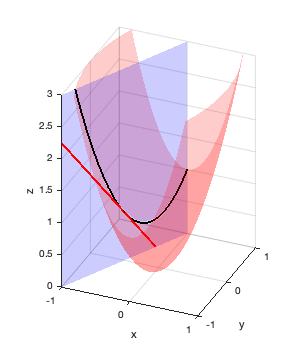
\includegraphics[scale=0.5]{img/C09tangent.png}
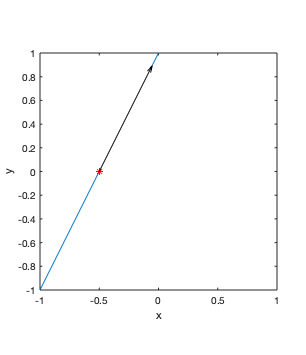
\includegraphics[scale=0.5]{img/C09tangentxy.png}

\begin{itemize}
\itemsep0em
    \item The directional derivative requires a point and a vector in the domain of $f(x,y)$.  (See plot on the right).
    \item The point is at $(x,y) = (-0.5, 2(-0.5)+1) = (-0.5,0)$.
    \item To find the vector direction, we have $y = 2x+1$ so $\Delta y = 2\Delta x$ and $\mb{u} = \langle 1, 2\rangle$.  The corresponding unit vector is $\hat{\mb{u}} = \mb{u}/\sqrt{5}$.
    \item $Df = (6x, 2y)$. $\left.Df\right\vert_{(-0.5,0)} = (-3,0)$
    \item The directional derivative is $\left.Df\right\vert_{(-0.5,0)} \hat{\mb{u}} = (-3,0)\left(\begin{array}{c} 1/\sqrt{5} \\ 2/\sqrt{5} \end{array}\right) = -3/\sqrt{5}$
\end{itemize}

The slope of the red line in the figure above is given by $-3/\sqrt{5}$.  For each unit of motion along the line $y = 2x+1$ in $xy$-space (with $x$ increasing), the $z$ value of the line moves down by $-3/\sqrt{5}$.


\vspace{0.2cm}
\hrule
\vspace{0.2cm}

\noindent\textbf{Example}

 Let $f(x,y,z)$ represent the temperature in degrees C at the point $(x,y,z)$ with $x,y,z$ in meters.  Assume you are moving at $\mb{v}$ meters per second through space.  (Instead of changing at unit rate, the inputs are changing at the rate given by \mb{v}).

The instantaneous rate of change of your temperature with respect to time is given by $[Df] \mb{v} = f_{\mb{v}}\Vert \mb{v}\Vert = \nabla f\cdot \mb v$

Identify the dimensions or units for each of $\Vert \nabla f\Vert$, $f_{\mb{v}}$, $\nabla f\cdot \mb{v}$, $\nabla f\cdot \hat{\mb{v}}$.
\vspace{1in}


%\item Let $f(x,y) = 3x^2+y^2$.  Construct a tangent plane to the graph of function about the point $(-1,1,4)$.


\begin{tcolorbox}
\begin{itemize}
    \item The \textbf{directional derivative} is sometimes described as the instantaneous rate of change of the function along the direction of $\mb{u}$ (where $\mb{u}$ is a vector in the domain of the function).
    \item Using the geometric definition of the dot product, $\left.f_{\mb{ u}}\right\vert_{(a,b)} = \left.Df\right\vert_{(a,b)}\hat{\mb{u}} = \left.\mb{\nabla}f\right\vert_{(a,b)}\cdot \hat{\mb{u}} = \Vert \mb{\nabla}f\Vert{(a,b)}\Vert\hat{\mb{u}}\Vert\cos\theta = \Vert \mb{\nabla}f\Vert_{(a,b)}\cos\theta$.
    \item At a point $(a,b)$, the directional derivative \textbf{has a maximum} (over all possible directions) $\Vert \mb{\nabla}f\Vert_{(a,b)}$ and a minimum of $-\Vert \mb{\nabla}f\Vert_{(a,b)}$.  The maximum occurs when $\mb{u}$ is a positive scalar multiple of $ \left.\mb{\nabla}f\right\vert_{(a,b)}$.
\end{itemize}
\end{tcolorbox}


\vspace{0.5cm}
\hrule
\vspace{0.2cm}

\noindent\textbf{Integration: single variable} 

\begin{tcolorbox}
\begin{itemize}
\itemsep0em
\item  Integrals are used to find totals, means, and other averaged quantities.  The relationship between wealth and income or between weight and food intake is an integral relationship (where one is the time integral of some function of the other).  Smoothing out noise in data is often done via integration (smoothing is an averaging process).
    \item A \textbf{definite integral}, $\int_{x=a}^b f(x)dx$, is defined in terms of a limit of Riemann sums.
    \item An \textbf{indefinite integral}, $\int f(x)dx$ is a class of functions (that are the same up to a constant), and is defined in terms of antiderivative.
    \end{itemize}
    \end{tcolorbox}
    \begin{tcolorbox}
    \begin{itemize}
    \itemsep0em
    \item Cut the interval $[a,b]$ into small subintervals of size $\Delta x$.  The sum $\displaystyle\sum\limits_{i}f(x_{i})\Delta x$, where $i$ indexes the intervals and $x_i$ is a point chosen from subinterval $i$, is called a \textbf{Riemann sum}, and is an approximation of the integral $\displaystyle\int_{x=a}^b f(x) dx$. (Riemann did this work around 1854.  It was published in 1867, after his death. \href{https://books.google.com/books?id=4JprCQAAQBAJ&pg=PA221&dq=riemann+sum+history&hl=en&sa=X&ved=0ahUKEwijlaKLgYbeAhVpk-AKHTHdCUkQ6AEIKTAA#v=onepage&q=riemann%20sum&f=false}{\color{blue}(Weblink to ``Elements of the History of Mathematics'')})
    \item For a function that is \textbf{Riemann-integral}, the limit of Riemann sums exists as $\Delta x \rightarrow 0^+$, and we have $\displaystyle\int_{x=a}^b f(x) dx = \lim\limits_{\Delta x\rightarrow 0^+} \sum\limits_i f(x_i) \Delta x$..
\end{itemize}
\end{tcolorbox}

\noindent\textbf{Examples}
\begin{enumerate}
    \item The Massachusetts Turnpike (“the Mass Pike”) starts in the middle of Boston and heads west. The number of people living next to it varies as it gets farther from the city.  Suppose that, $x$ miles out of town, the population density adjacent to the Pike is $P = f(x)$ people/mile. Express the total population living next to the Pike within 5 miles of Boston as a definite integral.
    \vspace{1cm}
    
    \item Provide an expression for finding the mean population density along the road.
    \vspace{3cm}
    
    \item The \textbf{center of mass} of an object lying along the $x$-axis between $x=a$ and $x=b$ is given by $\bar{x} = \int_a^b x \delta(x) dx / \int_a^b \delta(x)dx$ where   $\delta(x)$ is the density (mass per unit length) of the object.  Set up an expression to fin the center of mass of a $2$ meter rod if the density increases linearly from $0$ to $3$ kg/m along the length of the rod.
    \vspace{4cm}
    
    \item The \textbf{future value} of a payment $\$P$, is the amount to which $\$P$ would grow if deposited in an interest bearing account.  A common model is to assume that interest is compounded continuously (at interest rate $r$), so that the future value of an income stream of $P(t)$ dollars per year (for $M$ years, where $P(t)$ is in contemporary dollars at each time $t$) is given by $\int_0^M P(t)e^{r(M-t)}dt$, where money deposited at time $t$ has time $M-t$ to earn interest.  \emph{This is an example, with no question.}
    \vspace{0.5cm}
    
    \item Let $C$ be the region of the $x$-axis such that $-1\leq x \leq 1$.  By convention, $\int_C 1\ dx$ is positive (i.e. this notation indicates that the interval $C$ is being traversed in a `positive' direction).  Without calculating the integral, find the signs of
   $\displaystyle\int_C dx$,
    $\displaystyle\int_C x\ dx$,
   $\displaystyle\int_C (x-1)\ dx$. %\emph{pollQ}
   
   \vspace{2.5cm}
   
   \item Biological activity in a pond is reflected in the rate at which carbon dioxide is added or removed.  Plants take carbon dioxide out of the water for photosynthesis during the day and add it to the water at night (through respiration).  Animals put carbon dioxide into the water at all times.  The figure (taken from our textbook) shows the rate of change of carbon dioxide levels in a pond.  
   
   At dawn there were $2.600$ mmol of CO$_2$ per liter of water.
   
   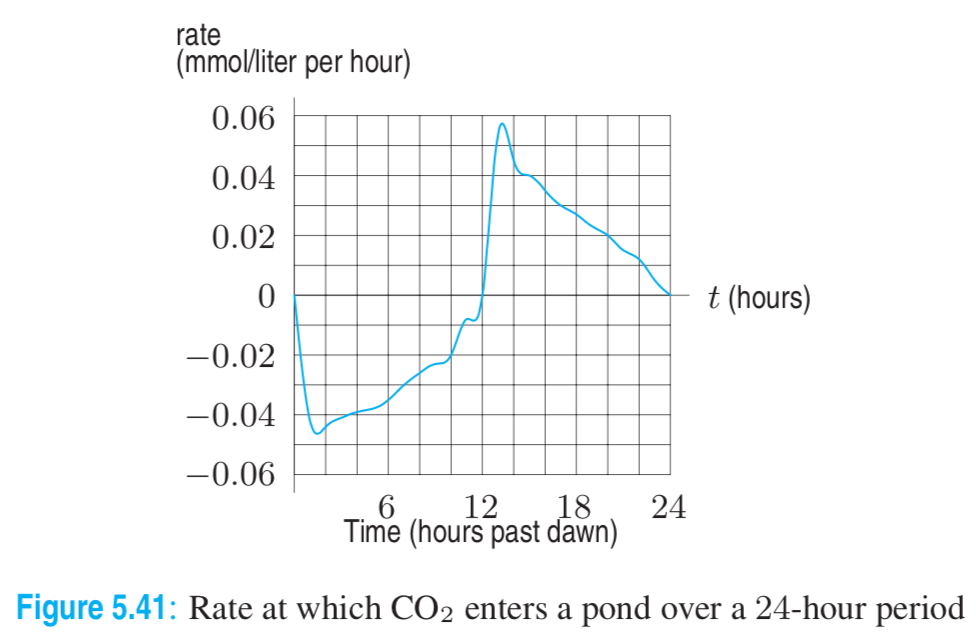
\includegraphics[scale=0.4]{img/C10pondco2.png}
   
   \begin{enumerate}
       \item At what time was the CO$_2$ level lowest?  What about highest?
       \vspace{1cm}
       
       \item Estimate how much CO$_2$ enters the pond during the night ($t = 12$ to $t = 24$).
      
      \vspace{3cm}
      
   \end{enumerate}
   
\end{enumerate}




\end{document}